\chapter{Results and Discussion}\label{chap:results_discussion}
\section{Results}\label{sec:results}
When evaluating the effectiveness of a binary prediction technique using a validation dataset with known activities, four central values are considered:

\begin{enumerate}
  \item True Positives (TP): The number of correctly predicted active cases.
  \item True Negatives (TN): The number of correctly predicted inactive cases.
  \item False Positives (FP): The number of incorrectly predicted active cases.
  \item False Negatives (FN): The number of incorrectly predicted inactive cases.
\end{enumerate}

Using these four values, it is possible to construct a confusion matrix and derive evaluation metrics, as illustrated in Figure~\ref{fig:confusion_matrix}:


\begin{figure} 
  \centering
  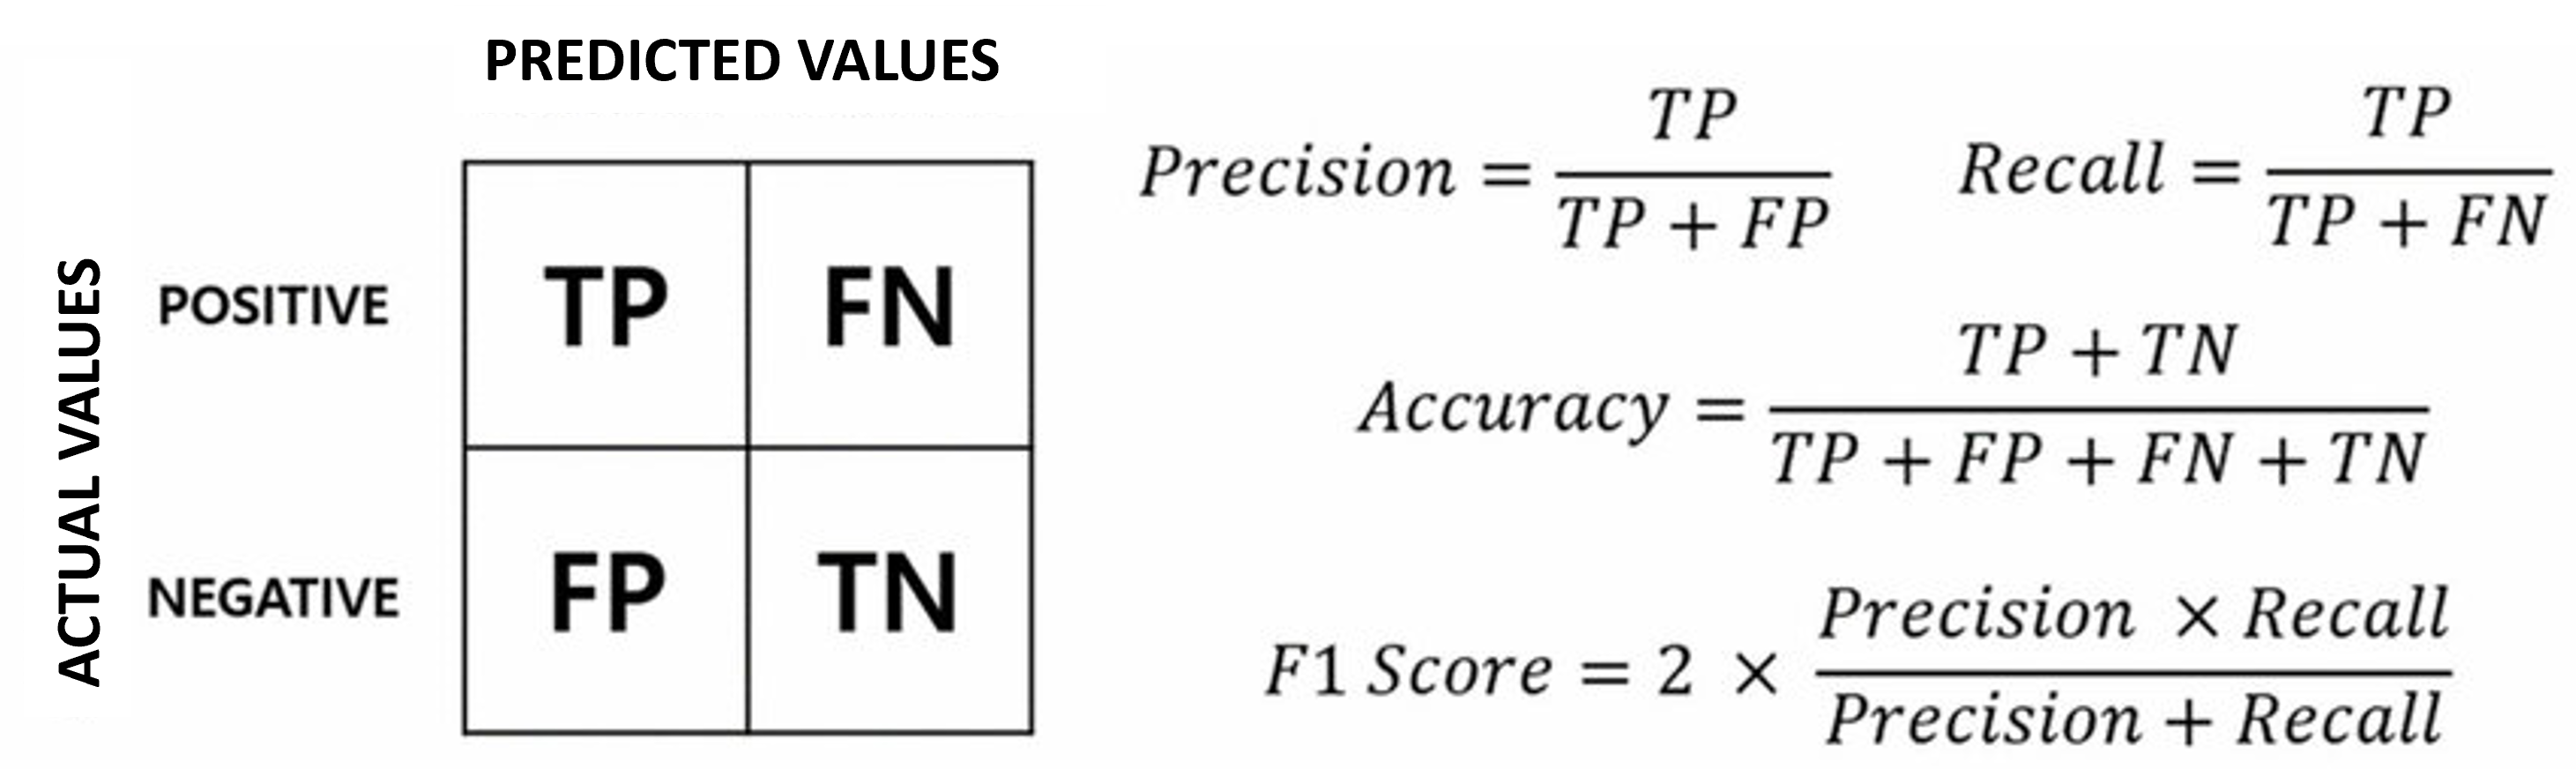
\includegraphics[width=1.0\textwidth]{figures/confusion_matrix_metrics.png}
  \caption{Confusion Matrix and Metrics: Accuracy, Precision, Recall, and F1 score.
  Figure obtained from~\cite{seol2023}.}
~\label{fig:confusion_matrix}
\end{figure}
\subsection{Evaluation}\label{sec:evaluation}
\section{Discussion}\label{sec:discussion}


